\chapter{Implementierung}
	Aus den oben beschrieben Überlegungen und dem in \cref{fig:flowchart} gezeigten grundlegenden Programmablauf folgt die nachfolgend beschriebene Implementierung in Software.



	\section{Vorbereitung der MCU}
		Um mögliche Fehlerquellen etwa durch \textit{cross-talking} auszuschließen, werden wie in \cite{MicrochipTechnologyInc.ATmega32U4.Datasheet.2016} auf Seite 71 beschrieben alle ungenutzten Pins in einen definierten Zustand -- hier als \textit{Input} mit aktiviertem \textit{Pull-Up} -- versetzt.
		Als Schnittstelle zum Touchscreen kommen nur Pins an Port F zum Einsatz welche vorbereitend ebenfalls als Input, allerdings ohne Pull-Up konfiguriert werden.\par

		Zur Umsetzung werden die Timer \texttt{Timer1} und bei Nutzung der internen ADC der obligatorische ADC-Timer verwendet.
		Letzter wird über einen eigenen Prescaler im Register \texttt{ADCSRA} konfiguriert.
		Um die volle Auflösung der ADC sicher ausnutzen zu können, darf die Frequenz des ADC-Timers gemäß Datenblatt \SI{200}{\kilo\hertz} nicht überschreiten.
		\begin{figure}[h]
			\centering
			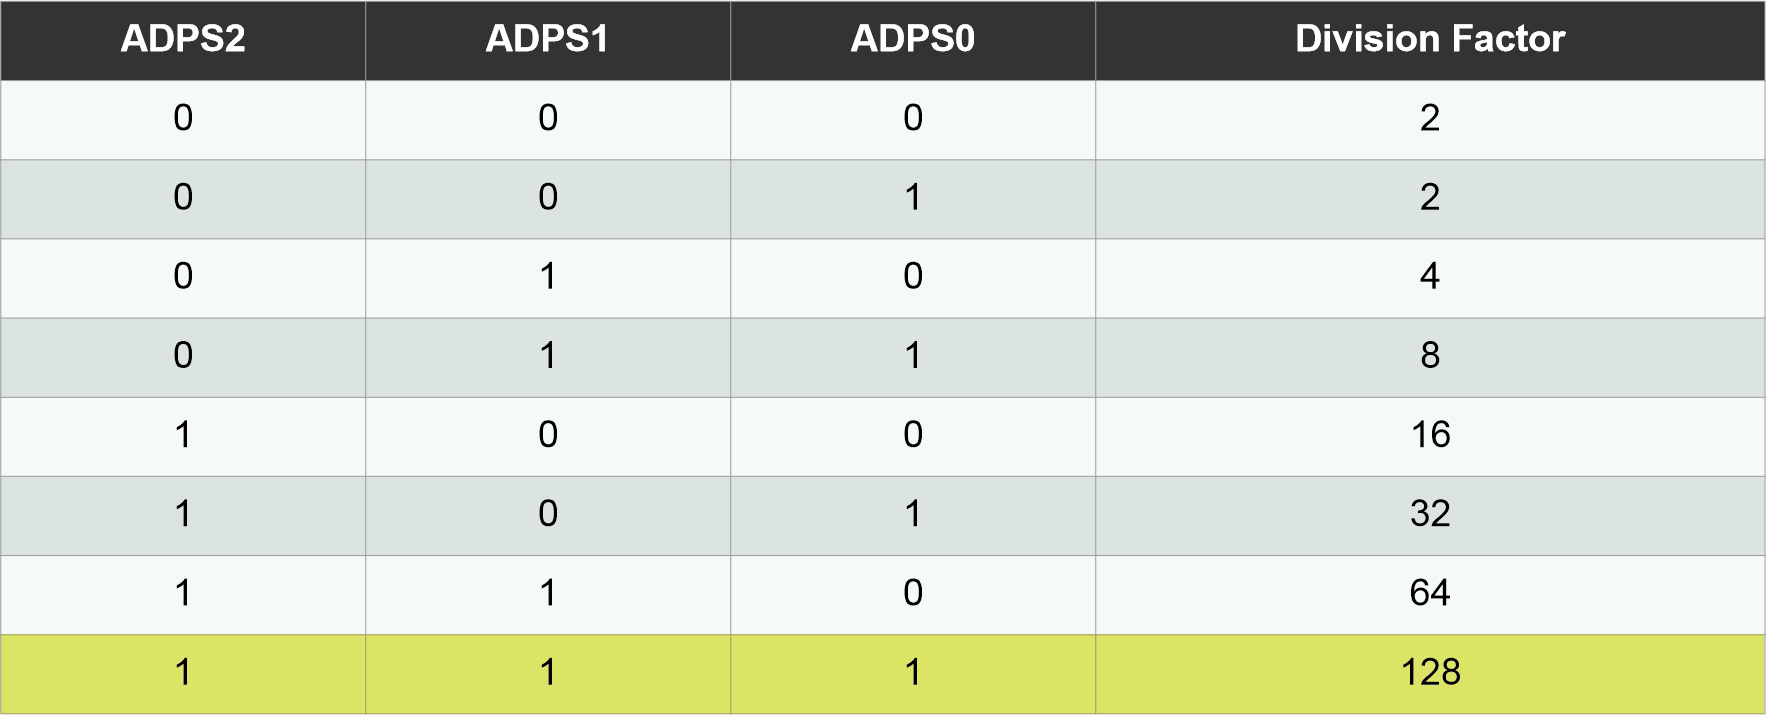
\includegraphics[width=.9\textwidth]{fig/ADC-Timer_Config.png}
			\caption[Auszug aus dem Datenblatt zu den relevanten Bits des Registers \texttt{ADCSRA}]{Auszug aus dem Datenblatt zu den relevanten Bits des Registers \texttt{ADCSRA} (Seite 316 \cite{MicrochipTechnologyInc.ATmega32U4.Datasheet.2016}).}
			\label{fig:adc timer konfig}
		\end{figure}
		Die möglichen Werte der Prescaler des ADC-Timers sind in \cref{fig:adc timer konfig} gezeigt.
		Mit der gelb hinterlegten Konfiguration errechnet sich die maximale ADC-Frequenz unter Beibehalt einer Auflösung von 10Bit zu
		\begin{equation}
			f_{ADC} = \frac{\SI{16}{\mega\hertz}}{128} = \SI{125}{\kilo\hertz}
			\label{eq:adc timer}
		\end{equation}
		was sich zu einer Periodendauer für einen Taktzyklus von \SI{8}{\micro\second} übersetzt.
		Weiter geht aus dem Datenblatt hervor, dass die Samplingdauer des ADC 1,5 Zyklen und die Konvertierungsdauer 13 Zyklen des ADC-Timers benötigt.
		Mit dem gewählten Prescaler ergibt sich so die benötigte Mindestdauer für eine Messung von
		\begin{align}
			t_{messung} &= t_{Sample} + t_{Hold} = \frac{n_{Sample}}{f_{ADC}} + \frac{n_{Hold}}{f_{ADC}} \nonumber \\
						&= \SI{14}{\micro\second} + \SI{102}{\micro\second} = \SI{116}{\micro\second}
			\label{eq:adc messdauer}
		\end{align}

		Dem Datenblatt des verwendeten Touchscreens ist zu entnehmen, dass mit einer maximalen Eingangsimpedanz zum ADC von \SI{850}{\ohm} (x-Richtung) zu rechnen ist \cite{FUJITSU.touchscreen.datasheet}.
		\cref{fig:analog input circuitry} zeigt die interne Eingangsverschaltung der ADC der verwendeten MCU. Die Kapazität \(C_{S/H}\) gilt es in der Zeit \(t_{Sample}\) auf einen Wert \(\frac{U_0}{2} \pm \frac{1}{2}LSB\) zu laden.

		\begin{gather}
			\frac{U_0}{2} - \frac{1}{2}LSB = U_0 \left( 1 - e^{-\frac{t_{Sample}}{RC}} \right) \nonumber \\
			\Leftrightarrow \nonumber \\
			t_{Sample} = -ln\left( \frac{1LSB}{2U_0} + \frac{1}{2}\right) \cdot RC
			\label{eq:samplingzeit}
		\end{gather}

		Mit Werten für \(R\), \(C_{S/H}\), \(U_0\) von \SI{850}{\ohm}, \SI{14}{\pico\farad} und \SI{5}{\volt} und \(\frac{1}{2}LSB = \frac{U_0}{2 \cdot 2^{10}}\) ergibt sich eine benötigte Samplingdauer von
		\begin{align}
			t_{Sample}	&= -ln\left( \frac{1}{2\cdot 2^{10}} + \frac{1}{2}\right) \cdot RC \nonumber \\
						&= -ln\left( \frac{1}{2\cdot 2^{10}} + \frac{1}{2}\right) \cdot \SI{850}{\ohm} \cdot \SI{14}{\pico\farad} \nonumber \\
						&= \SI{8,23}{\nano\second}
			\label{eq:samplingzeit gerechnet}
		\end{align}
		was sehr gut im Rahmen der gewählten ADC-Timerfrequenz liegt.
		Ebenso deckt es sich gut mit den Angaben des Datenblattes bei Eingangsimpedanzen unterhalb von \SI{10}{\kilo\ohm} seien Samplingzeiten vernachlässigbar.
		\begin{figure}[h]
			\centering
			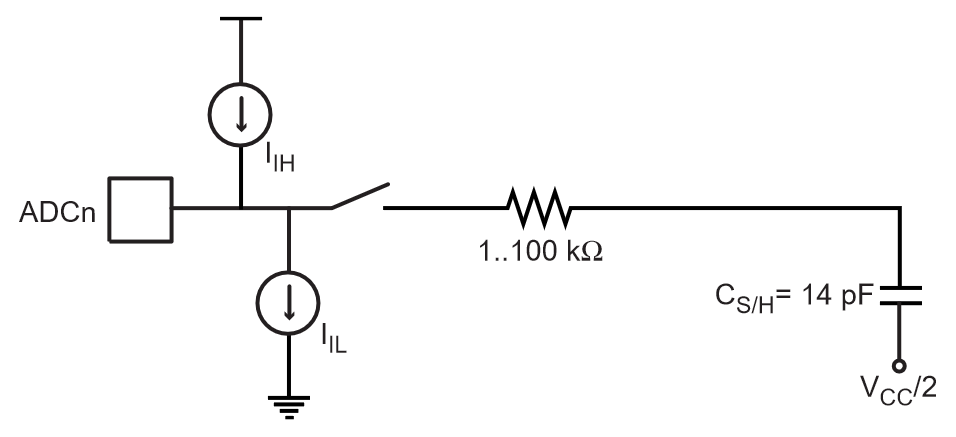
\includegraphics[width=.8\textwidth]{fig/adc-input-circuit.png}
			\caption[Interne Eingangsverschaltung der ADC]{Interne Eingangsverschaltung der ADC wie im Datenblatt gezeigt. Die Kapazität \(C_{S/H}\) ist hier der \textit{Sample and Hold}-Kondensator.}
			\label{fig:analog input circuitry}
		\end{figure}